%\documentclass[iop]{emulateapj}
\documentclass[aps, prl, twocolumn, groupedaddress, amsfonts, amssymb, amsmath]{revtex4-1}
\usepackage{graphicx}
\usepackage{bm}
\usepackage{natbib}
%\usepackage[colorlinks=True, linkcolor=blue, citecolor=blue]{hyperref}
%\usepackage[all]{hypcap}

\bibliographystyle{apsrev}

\newcommand{\Div}[1]{\ensuremath{\nabla\cdot\left( #1\right)}}
\newcommand{\angles}[1]{\ensuremath{\left\langle #1 \right\rangle}}
\newcommand{\grad}{\ensuremath{\nabla}}
\newcommand{\RB}{Rayleigh-B\'{e}nard }
\newcommand{\stressT}{\ensuremath{\bm{\bar{\bar{\Pi}}}}}
\newcommand{\lilstressT}{\ensuremath{\bm{\bar{\bar{\sigma}}}}}
\newcommand{\nrho}{\ensuremath{n_{\rho}}}
\newcommand{\approptoinn}[2]{\mathrel{\vcenter{
	\offinterlineskip\halign{\hfil$##$\cr
	#1\propto\cr\noalign{\kern2pt}#1\sim\cr\noalign{\kern-2pt}}}}}

\newcommand{\appropto}{\mathpalette\approptoinn\relax}

\begin{document}
%%%%% Create nice title and abstract
\author{Evan H. Anders}
\affiliation{Department of Astrophysical \& Planetary Sciences, University of Colorado -- Boulder}
\affiliation{Laboratory for Atmospheric and Space Physics, Boulder, CO}
\author{Benjamin P. Brown}
\affiliation{Department of Astrophysical \& Planetary Sciences, University of Colorado -- Boulder}
\affiliation{Laboratory for Atmospheric and Space Physics, Boulder, CO}
\title{Convective heat transport in stratified atmospheres at low and high Mach number}

\begin{abstract}
Here we study stratified convection in the context of 
plane-parallel polytropically stratified atmospheres. 
We hold the density stratification ($n_\rho$) and Prandtl number (Pr) constant while studying the dependence
of the Nusselt number (Nu), which quantifies the efficiency of convective heat transport, on
variations of the Mach number (Ma) and the Rayleigh number (Ra).  At large but still subsonic values of
Ma, a scaling $Nu \appropto Ra^{0.45}$ for low values of Ra.  As Ra increases and flows become supersonic,
this scaling gives way to a much weaker $Nu \appropto Ra^{0.20}$.  In the regime of $Ma \ll 1$, a consistent
$Nu \appropto Ra^{0.3}$ is retrieved,  reminiscent of the Nu $\propto$ Ra$^{2/7}$ seen in \RB convection.
\end{abstract}
\maketitle


%%%%% Body of the paper
\section{Introduction}
\refstepcounter{section}
\label{sec:intro}
Convection is essential to heat transport in the cores of high mass stars, the
envelopes of low mass stars, and the atmospheres of terrestrial and jovian planets. In such systems, convection
occurs in the presence of the atmospheric stratification, which can be small but extends up to 
14 density scale heights in the Sun's convective envelope.
A basic understanding of the
properties of compressible convection in stratified media is important to understanding systems in astrophysics
and planetary sciences.  Numerical constraints typically have restricted studies of stratified convection to
moderately high Mach numbers, appropriate to regions near the Sun's surface.  As such, we know little about the
fundamental properties of low-Mach number stratified convection, which occurs in the deep solar interior.

Some of the earliest numerical experiments on stratified convection
were performed in two \cite{graham1975, chan&all1982,
hurlburt&all1984, cattaneo&all1990} and three \cite{cattaneo&all1991, brummell&all1996} dimensions and
revealed a number of basic properties in the moderate-to-high Mach number regime.
In the widely-studied \RB (hereafter RB) problem, upflows and downflows are symmetrical and
the temperature gradient approaches zero in the convective interior causing the conductive flux to similarly 
disappear.  Highly stratified convection, on the other hand, exhibits narrow downflow lanes broad upflow regions.
Furthermore, the \emph{entropy} gradient is flattened by convection rather than the temperature gradient, which
means that even in the presence of perfectly efficient convection a significant component of the flux can be
carried by conduction.

In RB convection, there exist two primary control parameters: the Rayleigh number (Ra), the ratio of
buoyant driving to diffusive damping, and the Prandtl number (Pr), the ratio of viscous to thermal
diffusivity.  Along with the aspect ratio of the physical domain, these two numbers entirely control the
dynamics of the convection.  In stratified atmospheres, in addition to specifying the equation of state and
fundamental properties of the gas, the two control parameters of RB convection are joined by the degree of
stratification across the domain and the characteristic Mach number (Ma) of the convective flows.  
Polytropically stratified atmospheres, such as those used in early studies, are an ideal extension of
RB convection into the stratified realm as the two additional control parameters are directly linked to
basic properties of the atmosphere.  The density stratification is set by the number of density scale heights
the atmosphere spans (\nrho), and Ma is controlled by the superadiabatic excess ($\epsilon$),
the deviation of the polytropic index from the adiabatic polytropic index \cite{graham1975}.

In this letter we study the behavior of convective heat transport, quantified by
the Nusselt number (Nu), in polytropically stratified atmospheres.  
We vary $\epsilon$ and Ra while holding \nrho and Pr
constant across all simulations and convective structures which arise in a domain with an aspect ratio of 4.  In section 
\ref{sec:experiment}, we describe the construction of atmospheres, our equations, and our method for
numerical time evolution.  We describe our findings in section \ref{sec:results} and discuss
implications in section \ref{sec:discussion}.

\section{Experiment} 
\refstepcounter{section}
\label{sec:experiment}
In order to compare our results with previous studies and in an effort to examine a simplest case,
we study a fluid composed of monatomic ideal gas particles, with an adiabatic index of $\gamma = 5/3$ and
whose equation of state is $P = R^*\rho T$. 
The initial stratification is polytropic and the gravitational
acceleration and conductive heat flux are invariant throughout the depth of the atmosphere. We specify that both 
the thermal conductivity, $\kappa$, and the temperature gradient, $\grad T_0$, are constant while constructing
our atmosphere such that $\bm{F}_{\text{cond,0}} = -\kappa \grad T_0 = \text{constant}$.
Under these assumptions, solving the equation of hydrostatic equilibrium produces an atmosphere defined by
\begin{equation}
\begin{split}
\rho_0(z) &= \rho_{00}(z_0 - z)^m \\
T_0(z)    &= T_{00}(z_0 - z),
\label{eqn:polytrope}
\end{split}
\end{equation}
where $z$ increases upwards within the bounds $z =\{0, L_{z}\}$.
We specify the number of density scale heights the atmosphere spans, $n_\rho$, to determine $L_{z}$. Throughout
this letter, we set $n_{\rho} = 3$ such that the density at the bottom of the atmosphere is larger
than at the top by a factor of 20.
Thermodynamic variables are nondimensionalized at the top of the atmosphere as 
$P_0(L_z) = \rho_0(L_z) = T_0(L_z) = 1$, requiring $z_0 \equiv L_z + 1$ and $R^* = T_{00} = \rho_{00} = 1$.  
The polytropic index is set by the adiabatic index and the
superadiabatic excess, $\epsilon$, such that $m = m_{ad} - \epsilon$
where $m_{ad} \equiv (\gamma-1)^{-1}$ is the adiabatic polytropic index.
The subsequent entropy gradient at the top of the atmosphere is $\grad S(L_z) = -\epsilon$.  
The characteristic timescale of such an
atmosphere is related to the characteristic atmospheric buoyancy time, $t_{\text{b}} = \sqrt{L_z/g\epsilon}$.
We will utilize buoyancy time units throughout this letter.

Atmospheric diffusivities are set by the Rayleigh number and the Prandtl number.  We define the
non-dimensional Rayleigh number as
\begin{equation}
\text{Ra} = \frac{g L_z^3 (\Delta S_0 / c_P)}{\nu\chi},
\end{equation}
where $\Delta S_0$ is the entropy difference between the top and bottom of the atmosphere, 
$\nu$ is the kinematic viscosity (viscous diffusivity), and $\chi$ is the thermal dififusivity.  
The relationship between the thermal and viscous diffusivities is
set by the Prandtl number, Pr$ = \nu/\chi$.   We relate the dynamic viscosity, $\mu$, and the thermal conductivity,
$\kappa$, to their corresponding diffusivities such that 
$\nu \equiv \mu/\rho$ and $\chi \equiv \kappa/\rho$.  As a result, $\text{Ra} \propto (\nu\chi)^{-1} \propto
\rho^2$, such that for our atmospheres with $n_{\rho} = 3$, the Rayleigh number increases by a factor of
400 across the domain.  This formulation leaves Pr
constant throughout the depth of the atmosphere, and in this letter we impose $\text{Pr} = 1$.

At the constant values of $n_\rho$ and Pr used, the primary control parameters of convection are $\epsilon$
and Ra.  We decompose our atmosphere into the background polytrope ($\ln\rho_{0}, T_{0}$) and the fluctuations
about that background ($\bm{u}, \ln\rho_{1}, T_{1}$).  The scaling of the entropy gradient with $\epsilon$
is reflected in the evolved values of these fluctuations, which follow the scaling of
Ma$^{1/2} \propto T_1/T_0 \propto \rho_{1}/\rho_{0} \propto \epsilon$, and which scale as roughly $Ra^{0.25}$,
as in Fig. \ref{fig:ma_v_eps}.

\begin{figure}[t]
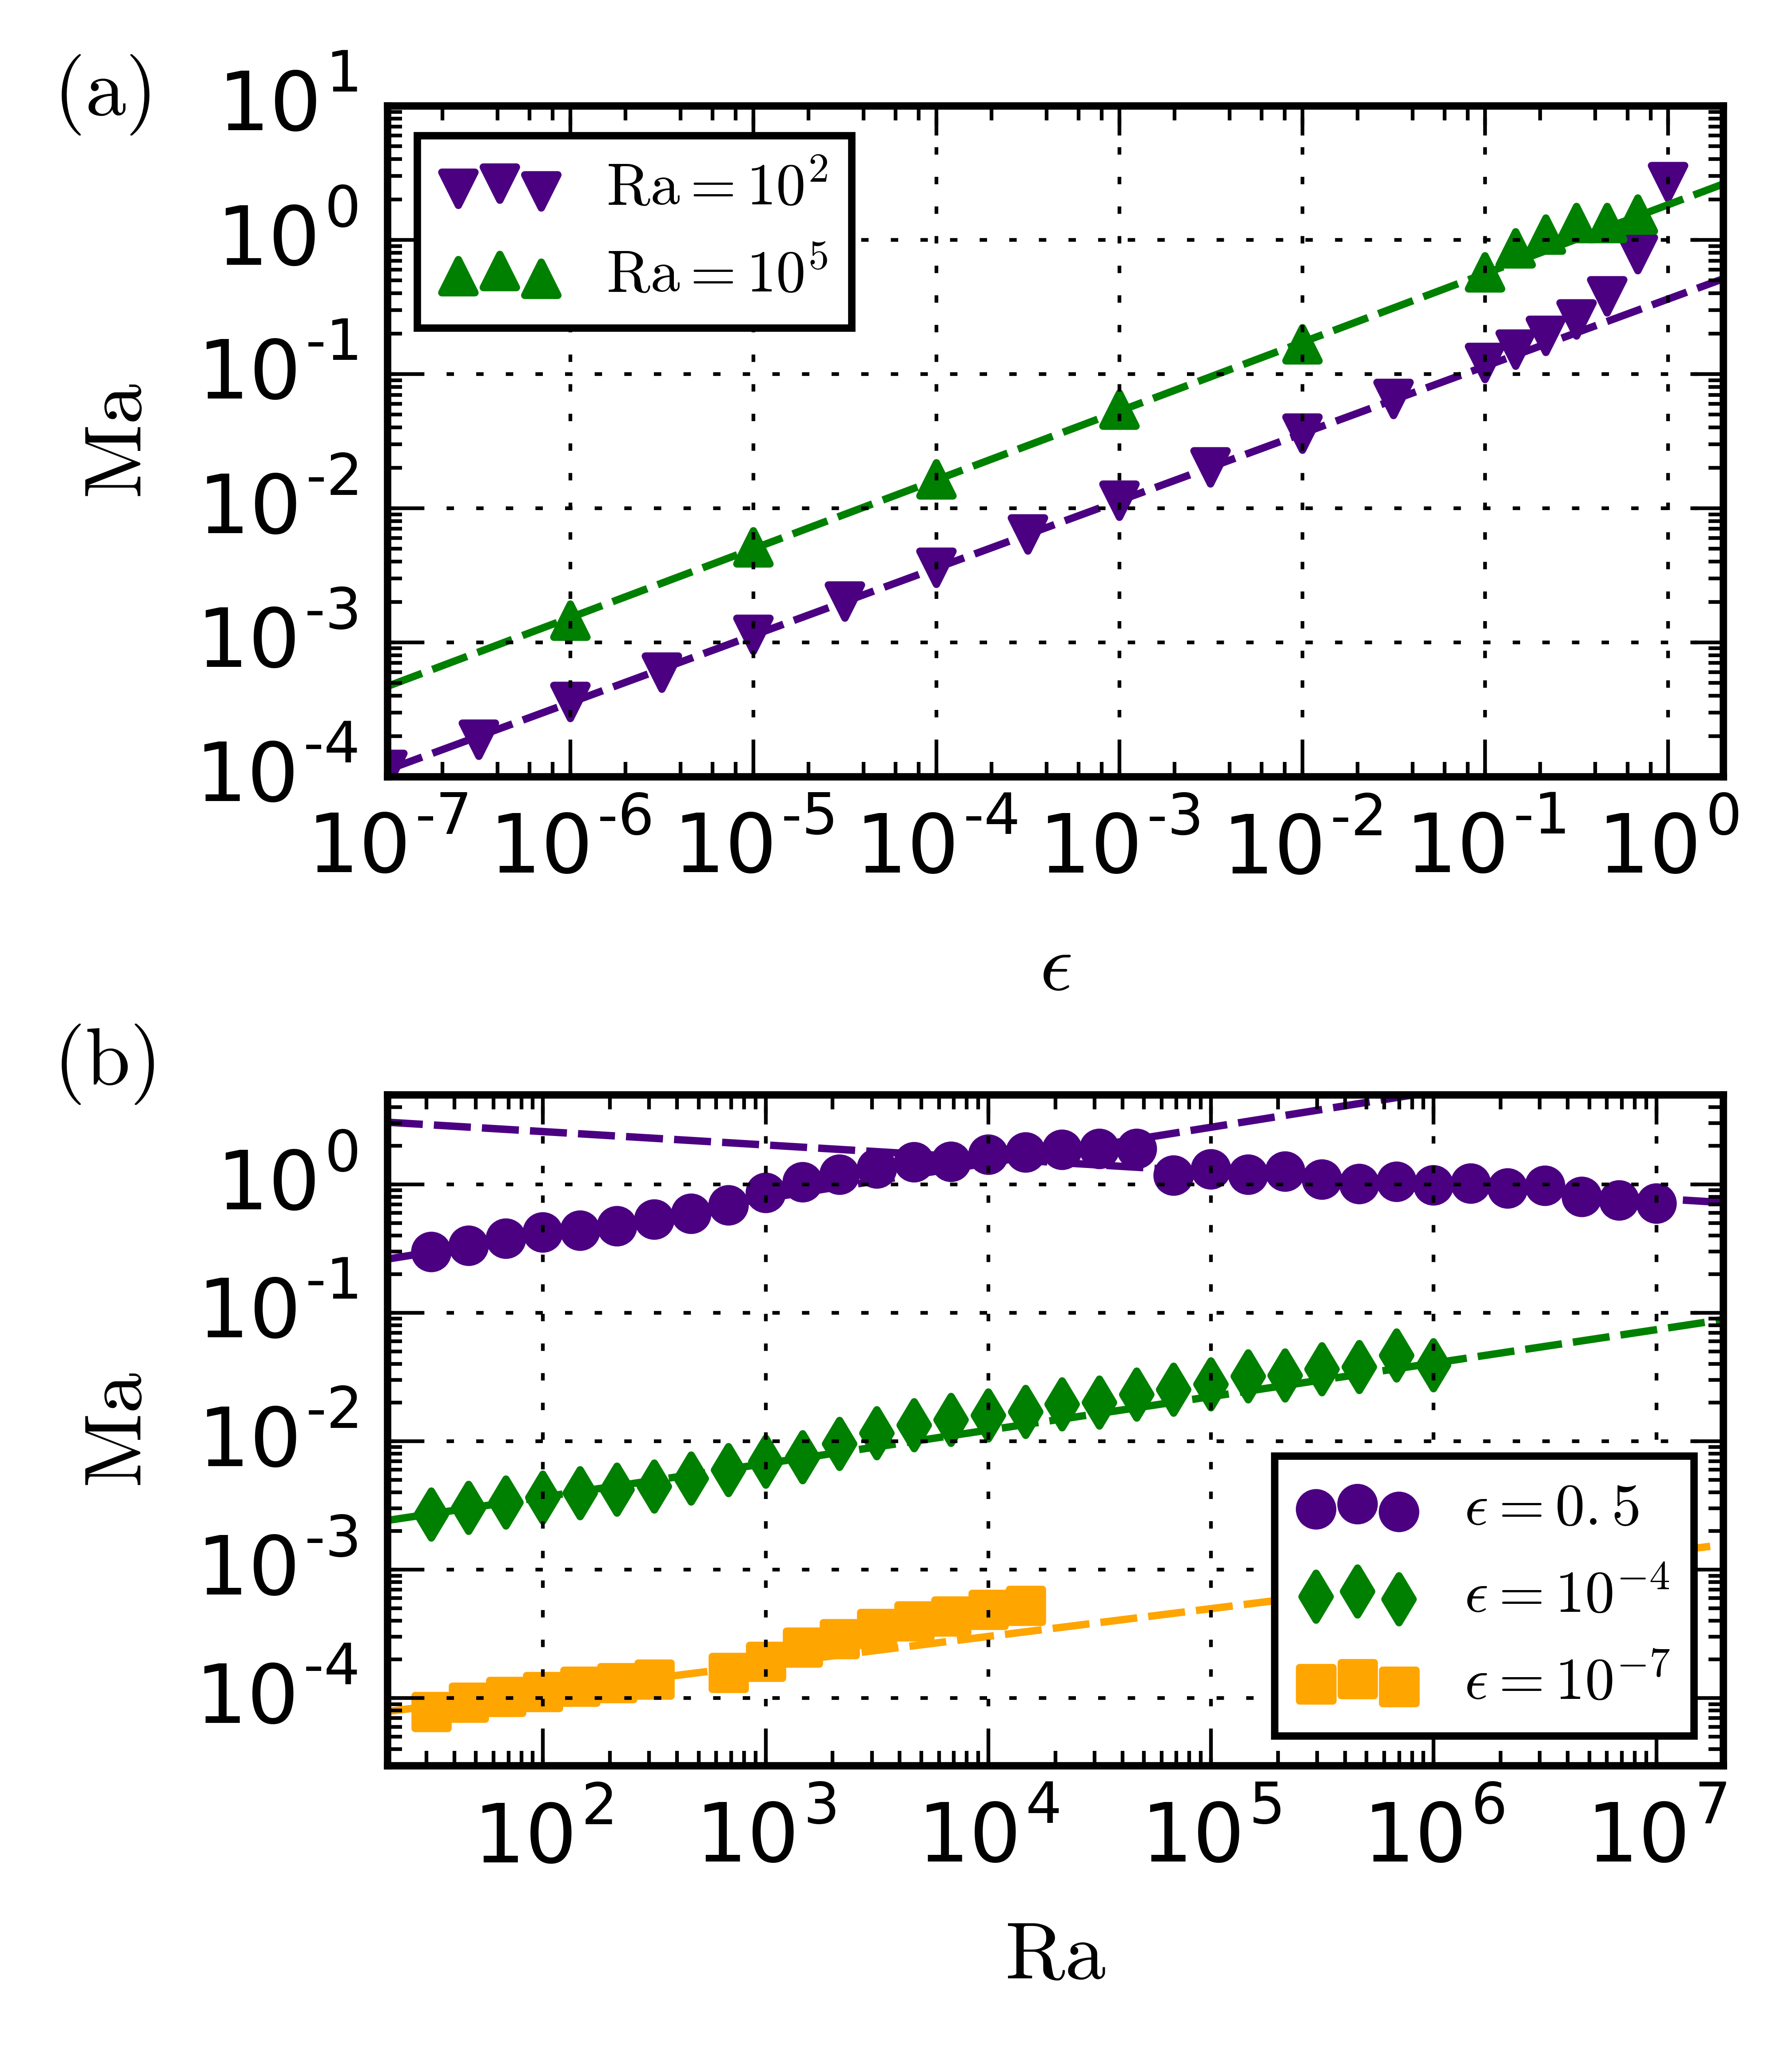
\includegraphics[width=3.4375in]{./figs/ma_v_eps.png}
\caption{(a) Characteristic horizontally averaged maximum Mach numbers which have been
time averaged for over 100$t_{b}$ starting roughly 50$t_{b}$ after the start of simulations. For $\epsilon \leq 0.1$,
an evident scaling of $Ma \propto \{\epsilon^{0.5015}, \epsilon^{0.5130}\}$ 
at Ra = $\{10^2, 10^5\}$ is retrieved.
When $\epsilon \rightarrow m_{ad}$, large deviations from this power law are seen and the system quickly
approaches Ma the supersonic regime.  
(b) At high epsilon, $Ma$ scales as $Ra^{0.2606}$ until it reaches the supersonic regime, at which point it turns
over and follows a power law of $Ra^{-0.1042}$.  At low epsilon, consistent power laws are achieved throughout all
values of $Ra$ studied, where $Ma \propto \{Ra^{0.2606}, Ra^{0.2165}\}$ for $\epsilon = \{10^{-4}, 10^{-7}\}$. All
error bars are negligible.  To study dynamics in the regime of deep solar convection ($Ma \approx 10^{-4}, 
Ra \approx 10^{20}$), a superadiabatic excess of $\epsilon \approx 10^{-17}$ is appropriate.
\label{fig:ma_v_eps} }
\end{figure}

We evolve the Fully Compressible Navier-Stokes equations,
which take the form:
\begin{align}
&\begin{aligned}
&\frac{D \ln\rho}{D t} = -\Div{\bm{u}}
	\label{eqn:continuity_eqn}
\end{aligned}\\
&\begin{aligned}
\frac{D\bm{u}}{D t}=
&-\grad T - T\grad\ln\rho + \bm{g} \\
&\,\,\,\,-\nu\Div{\lilstressT} - \lilstressT\cdot\grad\nu - \nu\lilstressT\cdot\grad\ln\rho
\label{eqn:momentum_eqn}
\end{aligned}\\
&\begin{aligned}
\frac{D T}{D t} = &-(\gamma-1)T\Div{\bm{u}} + \frac{\chi}{c_V}\grad^2 T + \\
&\grad T \cdot \grad\chi + \chi\grad T \cdot\grad\ln\rho +\nu\left(\lilstressT\cdot\nabla\right)\cdot\bm{u} 
	\label{eqn:energy_eqn}
\end{aligned}
\end{align}
where $D/Dt \equiv \partial_t + \bm{u}\cdot\grad$ and the viscous stress tensor is defined as
\begin{equation}
\sigma_{ij} \equiv \left(\frac{\partial u_i}{\partial x_j} + \frac{\partial u_j}{\partial x_i} - \frac{2}{3}\delta_{ij}\Div{\bm{u}}\right).
	\label{eqn:stress_tensor}
\end{equation}

In such stratified systems, the total convective flux can be defined as
\begin{equation}
\bm{F}_{\text{conv}} \equiv \bm{F}_{\text{enth}} + \bm{F}_{\text{KE}} + \bm{F}_{\text{PE}} + \bm{F}_{\text{visc}},
\end{equation}
where $\bm{F}_{\text{enth}} \equiv \rho\bm{u}(c_V T + P/\rho)$ is the enthalpy flux, $\bm{F}_{\text{KE}} \equiv 
\rho|\bm{u}|^2\bm{u}$ is the kinetic energy flux, $\bm{F}_{\text{PE}} \equiv \rho\bm{u}\phi$ is the potential
energy flux (with $\phi \equiv -gz$), 
and $\bm{F}_{\text{visc}} \equiv -\rho\nu\bm{u}\cdot\lilstressT$ is the viscous flux.  Taking an inner product of
Eq. \ref{eqn:momentum_eqn} with $\bm{u}$ and adding it to 
Eq. \ref{eqn:energy_eqn}, the full energy equation in conservation form is retrieved,
\begin{equation}
\frac{\partial}{\partial t}\left(\rho\left[\frac{|\bm{u}|^2}{2} + c_V T + \phi\right]\right) +
\Div{\bm{F}_{\text{conv}} + \bm{F}_{\text{rad}}} = 0
	\label{eqn:energy_eqn_full}
\end{equation}
where $\bm{F}_{\text{rad}} = -\kappa \grad T$.  An understanding of the flux terms is essential to characterizing
the convective heat transport in our systems.

The atmosphere is bounded above
and below by impenetrable, stress free, fixed temperature boundary conditions such that
\begin{equation}
w = \partial_z u = T_1 = 0
\end{equation}
at the boundaries. 

\textbf{Using a linear eigenvalue solve, we found the critical Ra number to be blahblahblah}


We utilize the novel Dedalus pseudospectral framework (http://dedalus-project.org/) to time-evolve Eqs. 
\ref{eqn:continuity_eqn}-\ref{eqn:energy_eqn} using an implicit-explicit third-order four-step 
Runge-Kutta timestepping scheme \cite{ascher&all1997}.  
Variables are time-evolved on a dealiased Chebyshev (vertical)
and Fourier (horizontal, periodic) domain in which the
physical grid dimensions are 3/2 the size of the coefficient grid.  Our physical grid sizes range from
96x384 grid points at the lowest values of Ra to 1152x4608 grid points at Ra $\geq 10^{7}$. 
By using IMEX timestepping, we are able to study flows at moderate ($Ma \approx 1$) and very low ($Ma \approx 10^{-4}$)
Mach number (Fig. \ref{fig:ma_v_eps}b).

\section{Results}
\refstepcounter{section}
\label{sec:results}

The efficiency of convection is quantified by the Nusselt number.  
While the Nusselt number is well-defined in RB convection
as the amount of total flux divided by the steady-state background conductive flux 
\cite{johnston&doering2009, otero&all2002},
a well-defined Nusselt number is more elusive in stratified convection.  A traditional definition of the Nusselt
number in stratified convection is \cite{graham1975,hurlburt&all1984}
\begin{equation}
Nu \equiv \frac{F_{\text{conv, z}} + F_{\text{rad, z}} - F_A}{F_{\text{ref}} - F_A},
\label{eqn:nusselt}
\end{equation}
where $F_{\text{conv, z}}$ and $F_{\text{rad, z}}$ are the z-components of $\bm{F}_{\text{conv}}$ and $\bm{F}_{\text{rad}}$,
respectively.  $F_A$ is the adiabatic conductive flux, defined as $F_A = -\kappa \partial_z T_{\text{ad}}$.  For an
ideal gas atmosphere in hydrostatic equilibrium, $\partial_z T_{\text{ad}} \equiv - g / c_{P}$.
$F_{\text{ref}} = \Delta T / L_z$ , where $\Delta T = T_{u} - T_{\ell}$, is the conductive flux of a linear profile connecting the upper
and lower plates.

We contend that this is the general form of the Nusselt number.  To illustrate this, we consider a few limiting
cases. Convection works to
suppress entropy stratification and create isentropic atmospheres.  Under the Boussinesq approximation,
density variations are ignored and entropy stratification is directly proportional to temperature stratification,
such that $\grad S \rightarrow 0$ only when $\grad T \rightarrow 0$.  Thus, for RB convection, 
$\grad T_{\text{ad}} \equiv 0$ and the familiar form of $Nu$ is retrieved.  In the case of stratified convection,
as $\epsilon \rightarrow m_{ad} + 1$, $\grad P \propto g \rightarrow 0$ and
the resulting $\grad T_{\text{ad}} \rightarrow 0$.  In such a case, $F_A \rightarrow 0$ and the familiar
definition of the RB Nusselt number is appropriate to use, as convection carries all of the
atmospheric flux in such a case \cite{brandenburg&all2005}. As $\epsilon \rightarrow 0$, 
$\grad T_{\text{ad}}\rightarrow \grad T_0$, the atmospheric initial temperature profile.  This causes increasingly
smaller velocity, and thermodynamic perturbations (e.g. Fig. \ref{fig:ma_v_eps}), but the removal of the 
O(1) background term in the numerator and denominator of Eq. \ref{eqn:nusselt}, makes the numerator and
denominator both O($\epsilon$).

We solved initial value problems which start in hydrostatic and thermal equilibrium and experienced infinitesimal 
kicks compared to $\epsilon$ in $T_1$.  Solutions were time-evolved until a long-time average of $Nu$ showed little
dependence on height. At
high values of $\epsilon$, shock systems form in the upper atmosphere near downflow lanes 
(see e.g. Fig. \ref{fig:entropy_snapshots}a) and propagate towards upflow lanes.  Such systems were reported in
both two \cite{cattaneo&all1990} and three \cite{malagoli&all1990} dimensional polytropic simulations previously.
It is unsurprising that \cite{cattaneo&all1990} discovered that as $\gamma \rightarrow 1$, shocks are easier to
find and produce, as in such a regime $m_{ad} \rightarrow \infty$ and, as a result, $\epsilon \rightarrow \infty$.
Low mach number flows, such as those in an $\epsilon = 10^{-4}$ atmosphere (e.g. Fig. \ref{fig:entropy_snapshots}b)
have similar bulk thermodynamic structure but lack the complicating dynamics of shock heating. This is interesting
in light of the current literature, as low Mach number flows are in pressure equilibrium with the background and
so pressure forces can no longer be the cause of narrow downflow lanes and broad upflow regions, as suggested
by \cite{hurlburt&all1984}.  As Ra is
increased to very large values (e.g. Fig. \ref{fig:entropy_snapshots}c), thermodynamic structures 
break up into small packets which traverse through the domain many
times before diffusing rather than spanning the whole domain.  
The complicated nature of high Ra dynamics, especially in the low Ma regime where
shocks are absent, has barred us from sufficiently converging any solutions in the regime of $Ra > 10^6$
at low $\epsilon$.

\begin{figure}[t]
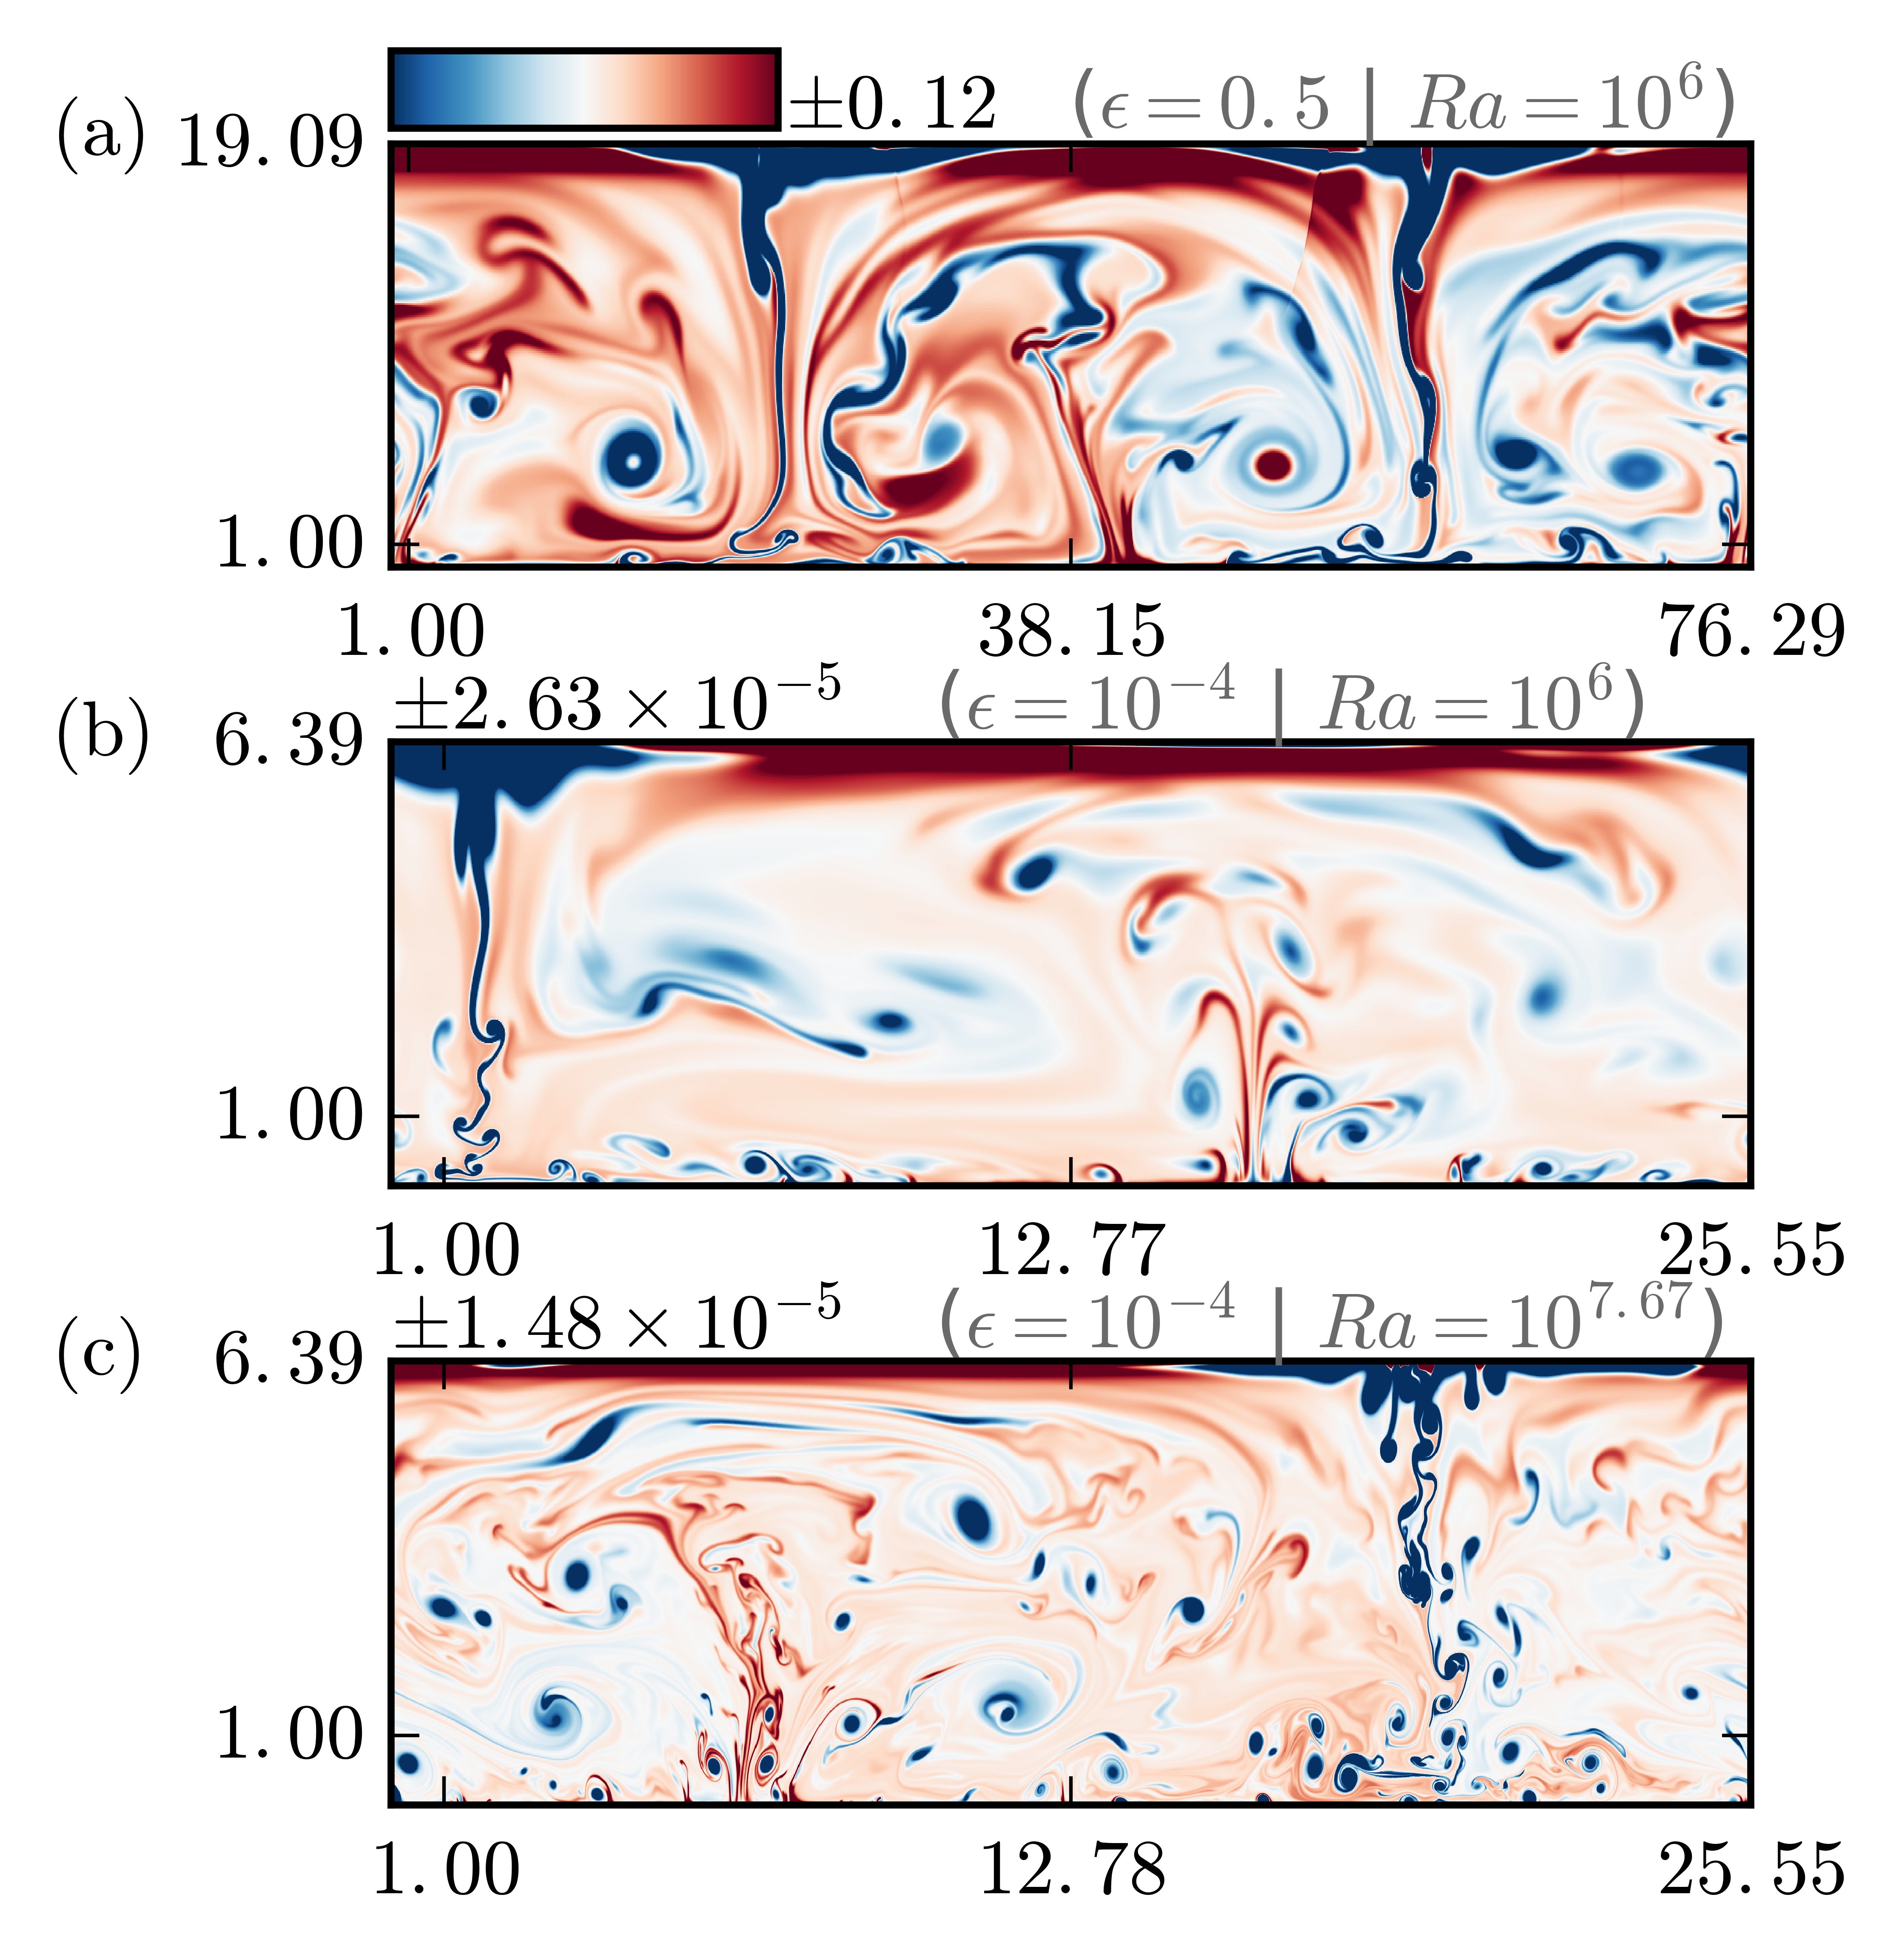
\includegraphics[width=3.4375in]{./figs/snapshots_fig.png}
\caption{Characteristic entropy. The time- and horizontally-
averaged profile is removed in all cases.  At high
$\epsilon$ (a), shock systems form near the upper downflow lanes and propel shock-heated material deep within
the atmosphere at sufficiently high Ra.  At low $\epsilon$ but at the same Ra (b), shock systems are absent, 
but otherwise the dynamics are similar.  As Ra is increased (c), downflow lanes no longer span
the entirety of the domain and individual small blobs are responsible for carrying the flux.
\label{fig:entropy_snapshots} }
\end{figure}

At high values of Ra, the heat transport properties of the systems become increasingly complex and time-dependent.
Large $\epsilon$ flows exhibit two local maxima in the enthalpy flux and kinetic energy flux: one in the upper 
atmosphere caused by the shocks, and one in the lower atmosphere caused by the deep mixing of convective motions.
At low $\epsilon$, only the deep maximum is present.  Furthermore, for low values of $\epsilon$, the presence
of fixed-temperature boundary conditions allows the flux at the boundaries to vary.  Many runs at $Ra > 10^5$,
$\epsilon = 10^{-4}$ exhibit time-dependent states of stratified convection (such as those shown in 
Fig. \ref{fig:entropy_snapshots}), in which the flux entering the system at the bottom of the atmosphere exceeds
that at the top.  These states are punctuated by states of vigorous shearing which flatten the bottom temperature
gradient towards adiabatic, allowing the excess energy to exit through the upper boundary.  These shearing
states will be covered in more detail in a future paper.  Regardless, a proper long-term average over shearing
and non-shearing states retrieves an invariant flux profile (and therefore Nu profile) throughout the depth
of the atmosphere (\textbf{After about 24 more hours, it'll be flat!  I don't have enough data at the parameters
shown in Fig. \ref{flux_profiles} yet}).

\begin{figure}[t]
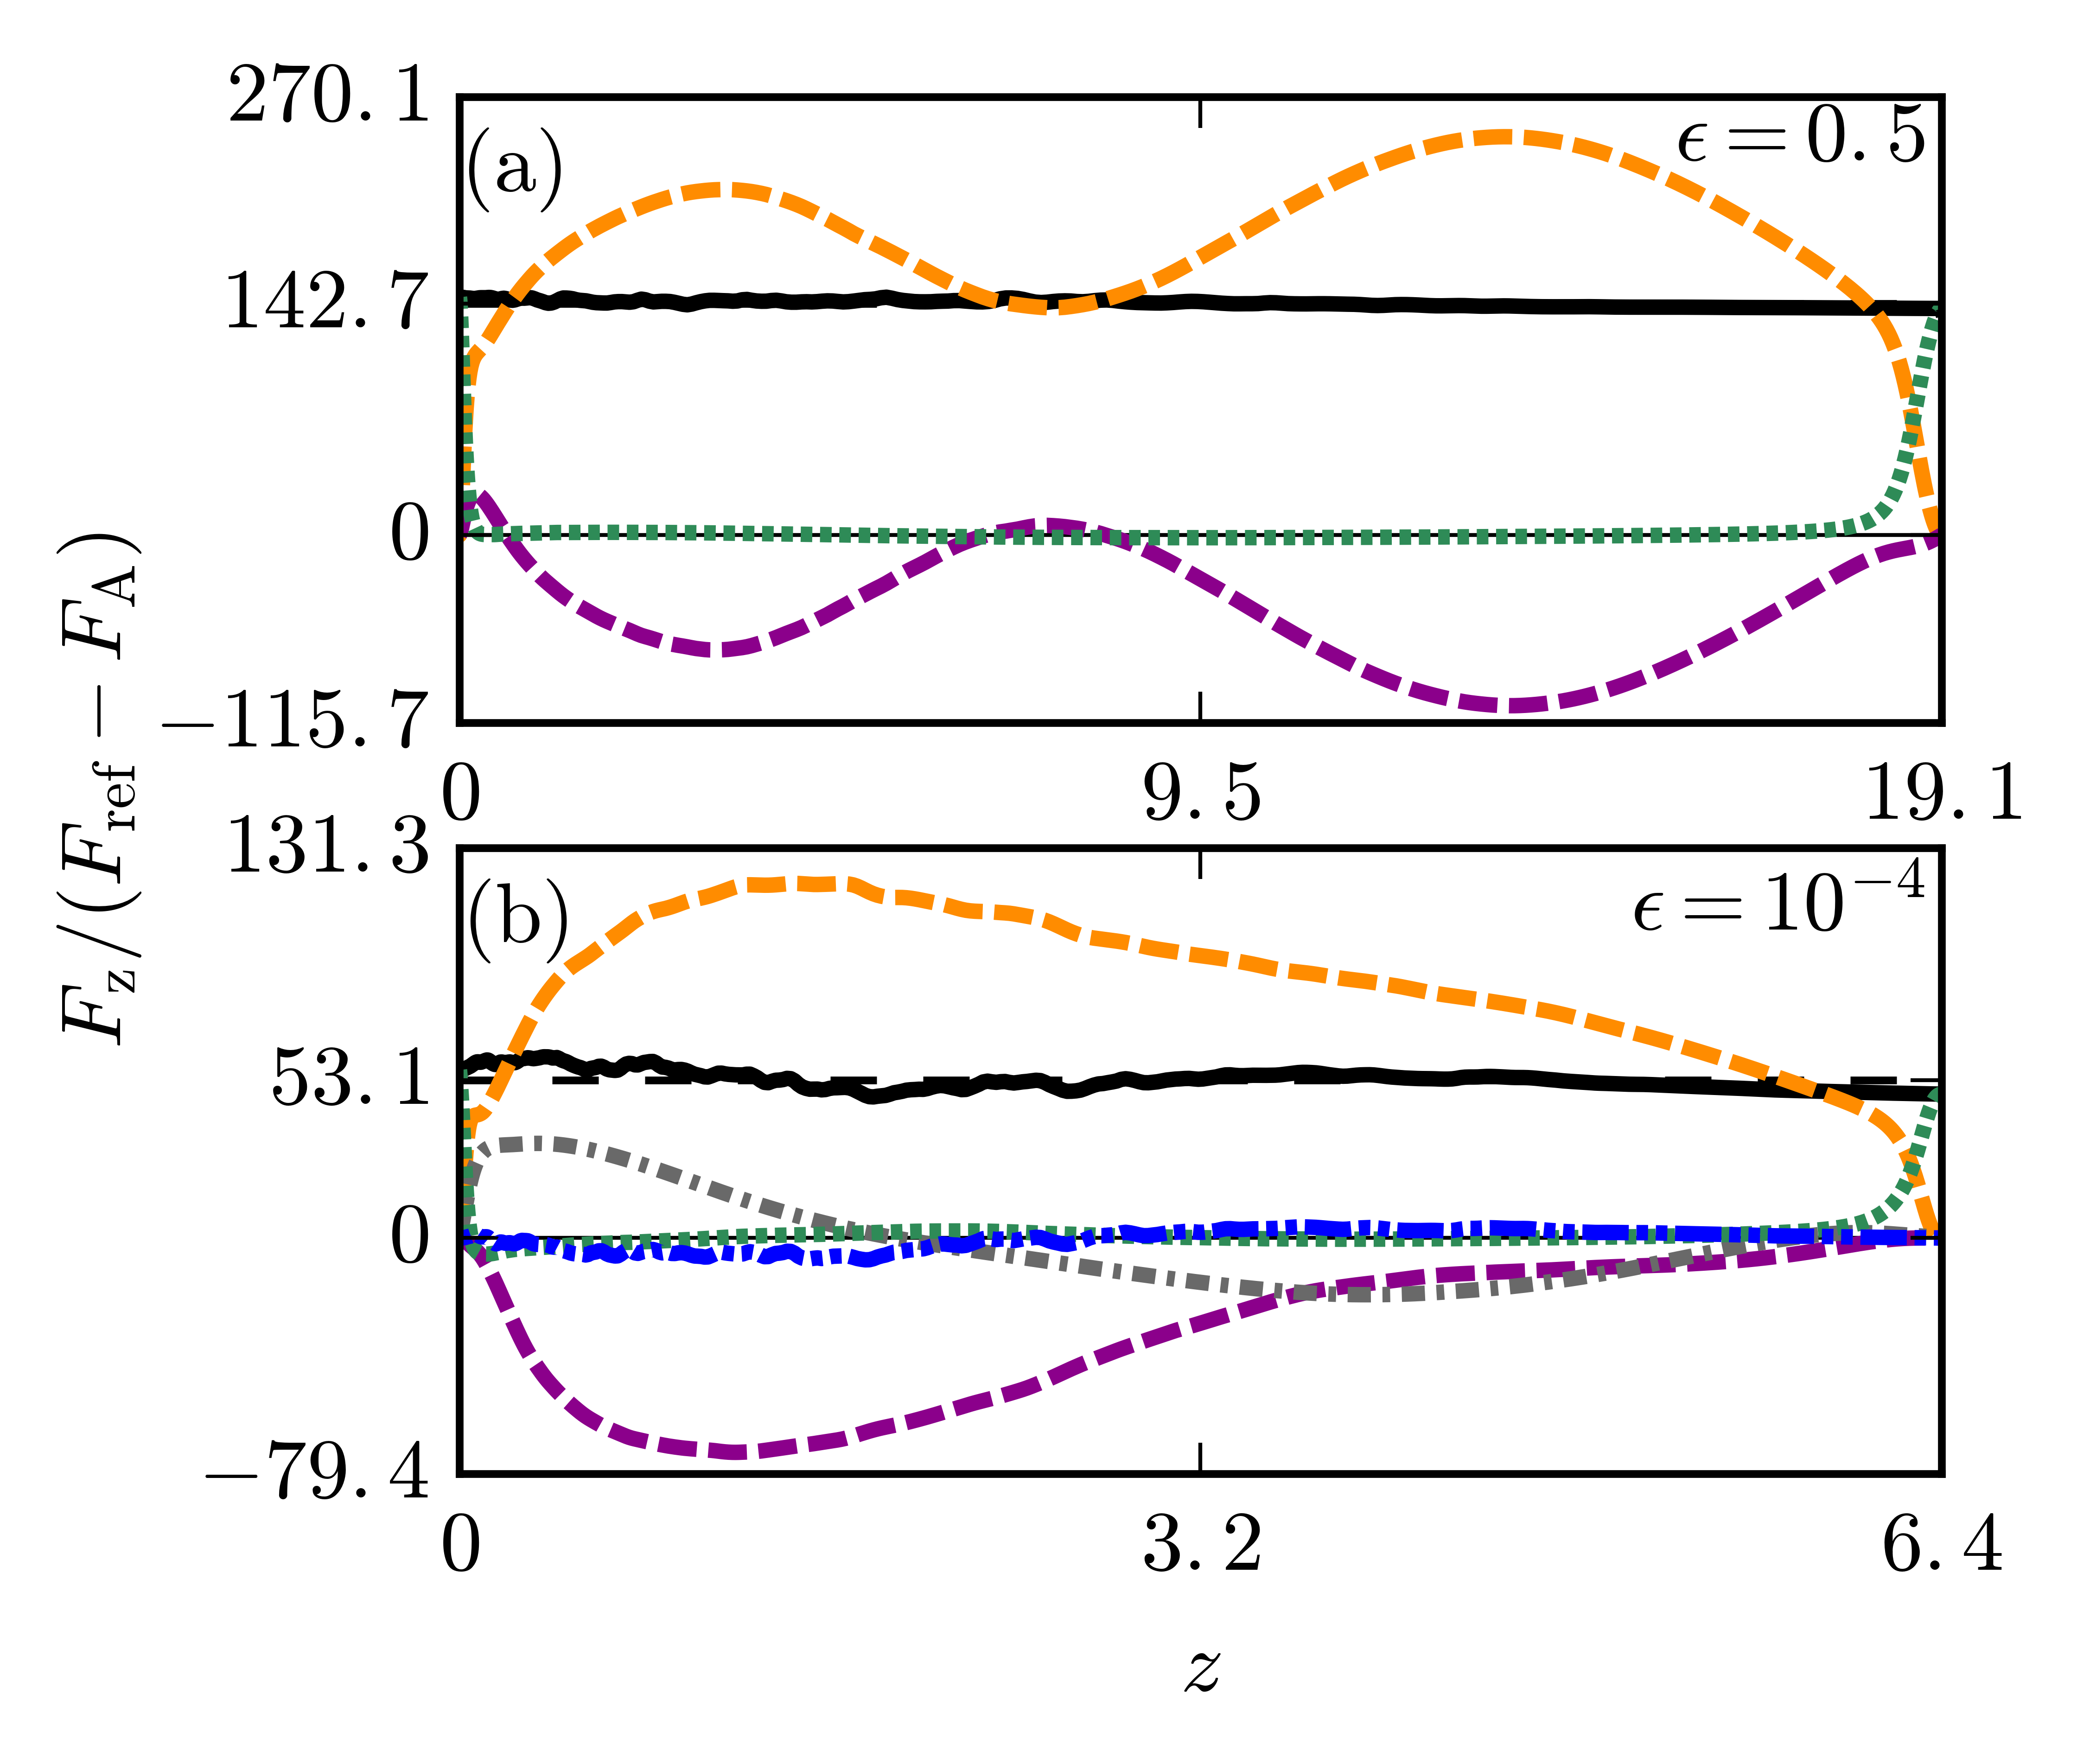
\includegraphics[width=3.4375in]{./figs/fluxes_fig.png}
\caption{Time-averaged flux profiles for low (top) and high (bottom) Mach number flows at $Ra = 10^6$.  
The dashed lines correpond to the
enthalpy flux (orange, positive) and kinetic energy flux (purple, negative).  The grey dash-dot line is the
viscous flux, and the green dotted line is the radiative flux with the adiabatic radiative flux removed. All
fluxes are normalized by $F_{ref} - F_A$, as in the calculation of the Nusselt number.  The solid black line is
the properly normalized sum of all the fluxes, and under this normalization its height-averaged value is the
Nusselt number.
\label{fig:flux_profiles} }
\end{figure}

After appropriately time-averaging the fluxes, a sensible Nusselt number is retrieved.  Nusselt numbers for
all simulations at low and high Ma are plotted in Fig. \ref{fig:nu_v_ra}.  At $\epsilon = \{10^{-4}, 10^{-7}\}$,
scaling laws of $Nu \propto Nu^{\{0.3090, 0.3087\}}$ are retrieved.  At $\epsilon = 0.5$, in the near-sonic
regime ($Ra \leq 10^4$), the scaling of $Nu$ with $Ra$ is inflated, with $Nu \propto Ra^{0.4489}$.  As simulations
pass into the supersonic regime and shocks start to form near the downflows, propoelling warm fluid deep
into the atmosphere, that scaling drops to $Nu \propto Ra^{0.1936}$.  Error on all power law scalings is
negligible.

\begin{figure}[t]
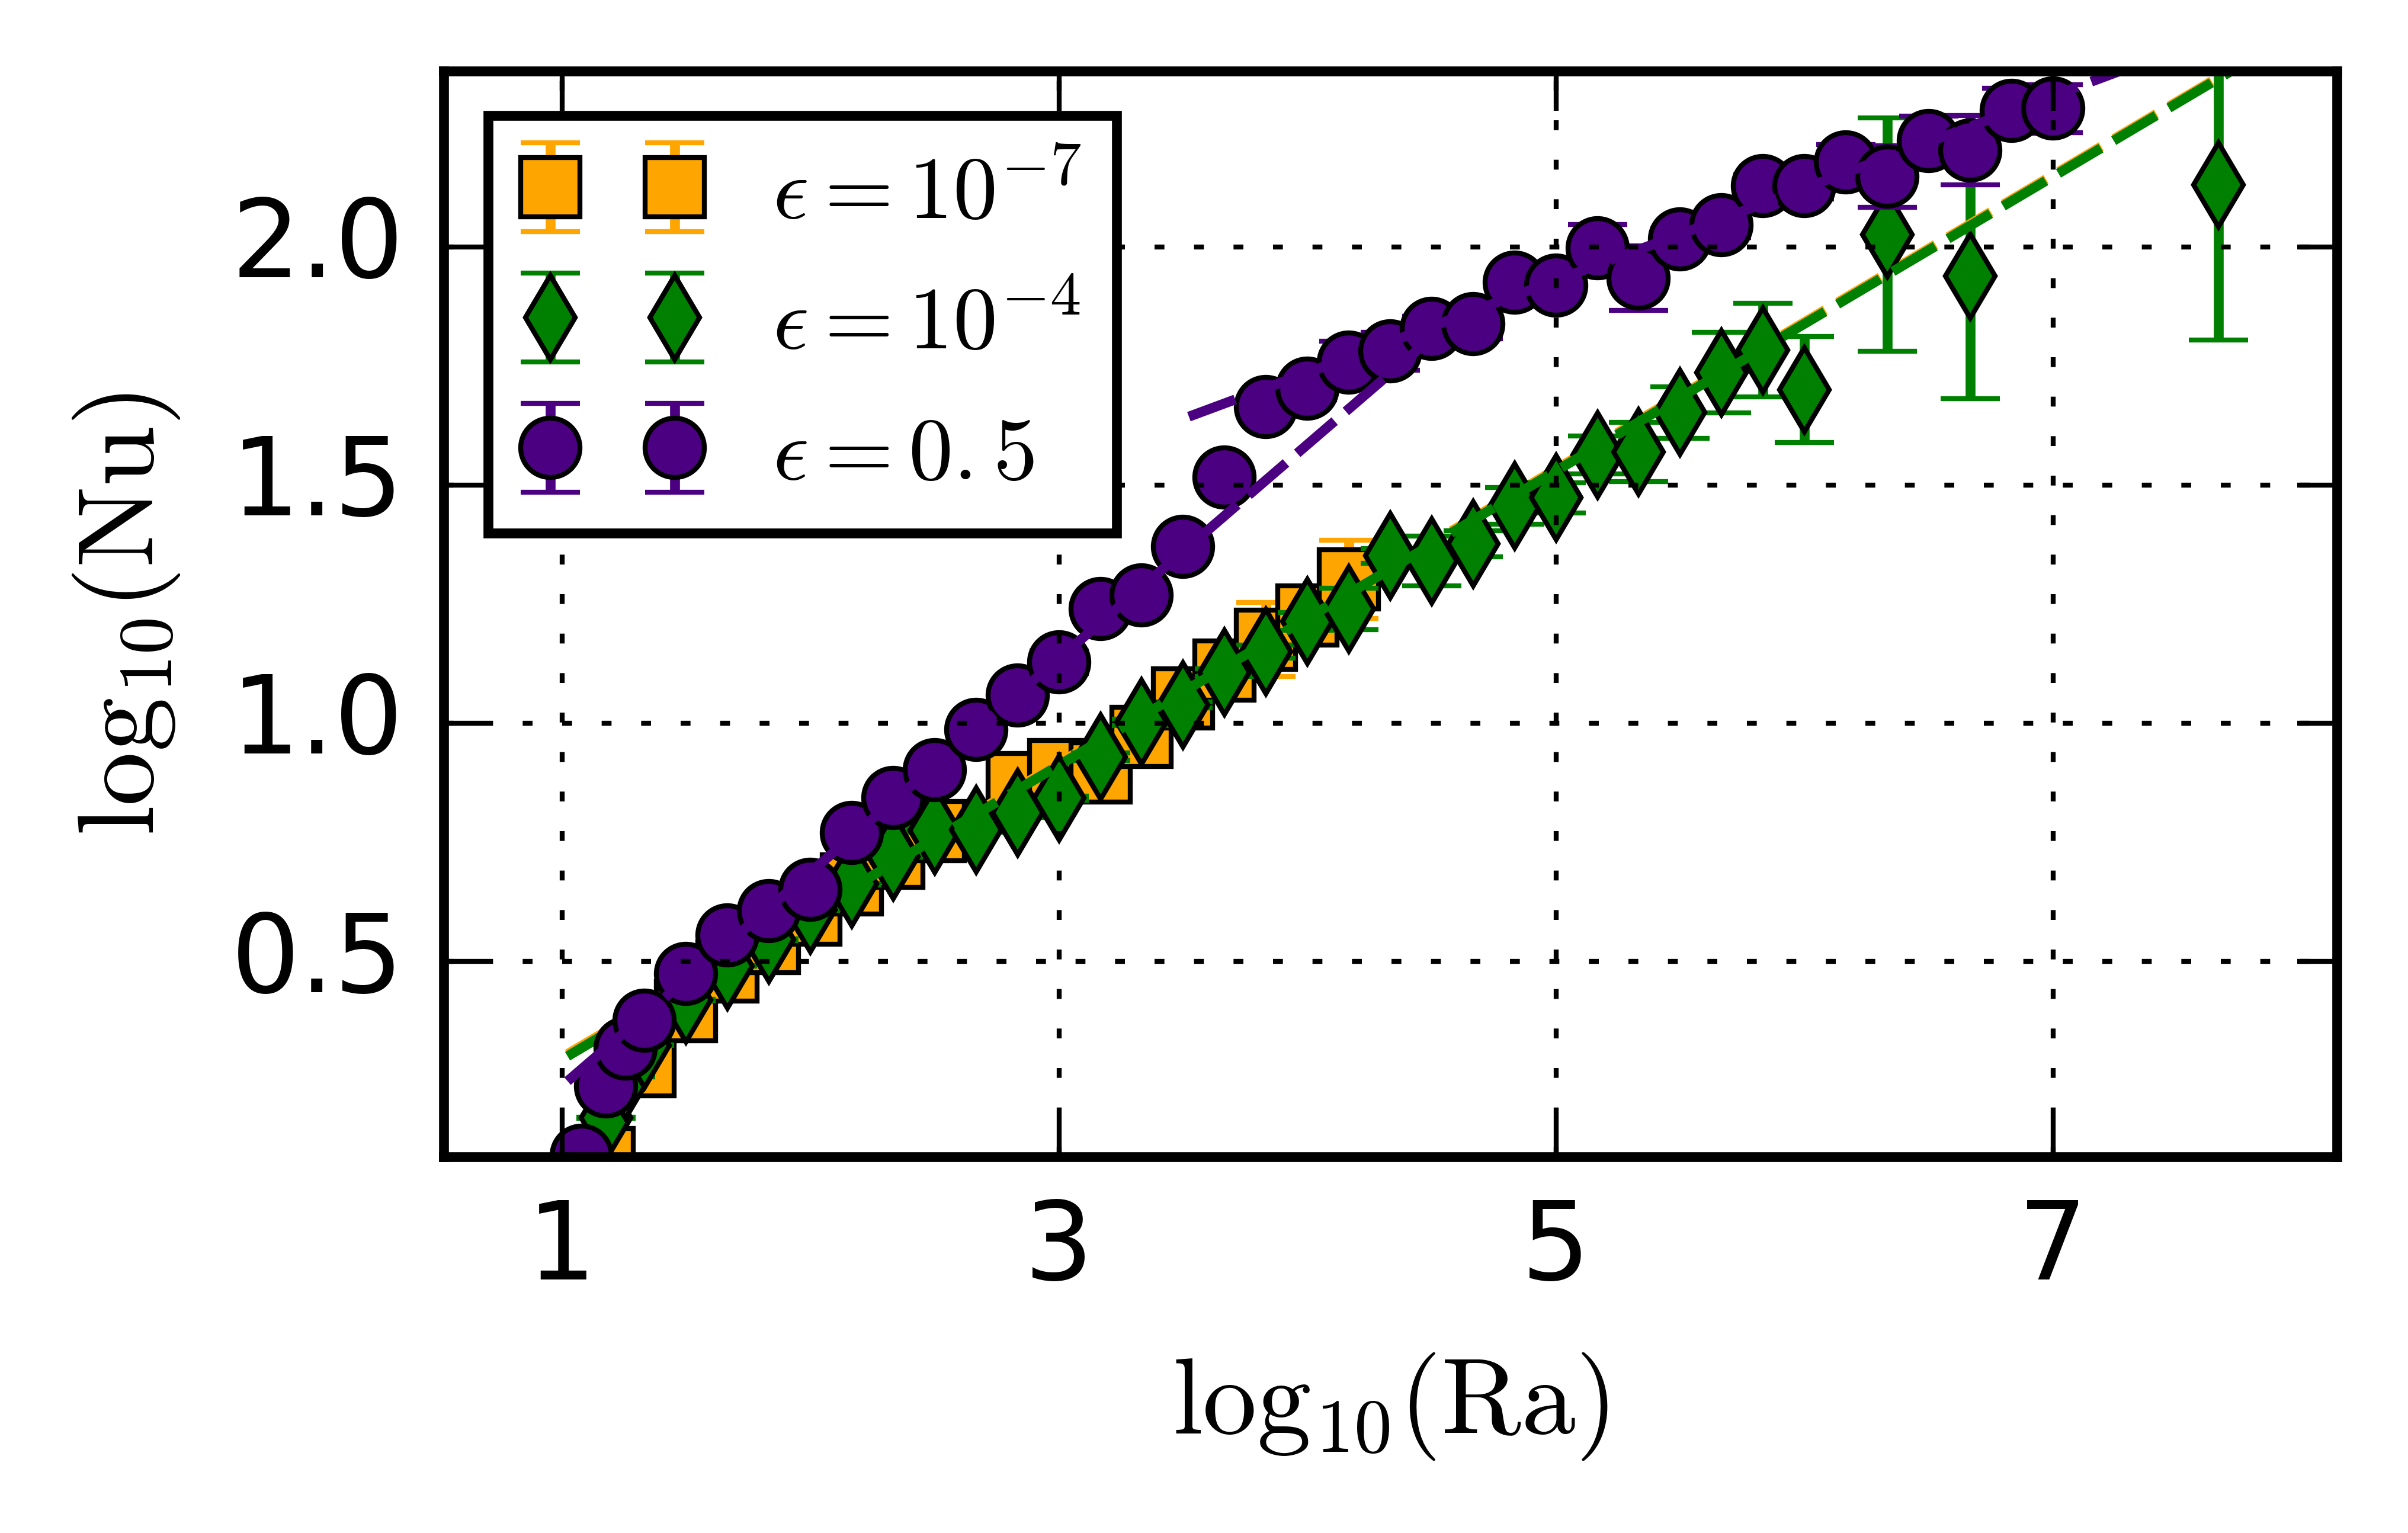
\includegraphics[width=3.4375in]{./figs/nu_v_ra.png}
\caption{Variation of $Nu$ as $Ra$ increases is shown for $\epsilon = \{10^{-7}, 10^{-4}, 0.5\}$. 
At high $\epsilon$, a clear transition from the subsonic to supersonic regime is evident in the scaling
of Nu with Ra.  In the low $\epsilon$ regime Nu vs. Ra scalings collapse onto a similar line which is
reminiscent of RB scalings \cite{johnston&doering2009}.
\label{fig:nu_v_ra} }
\end{figure}

\section{Discussion}
\refstepcounter{section}
\label{sec:discussion}
Here we have presented a non-dimensional construction of polytropic atmospheres and the control parameters 
which determine flow characteristics in such systems.  We argue that such systems are the natural extension
of the RB problem to stratified systems, and should be used to understand the basic properties of stratified
convection.  We have argued that the traditional definition of the Nusselt number in stratified atmospheres
\cite{graham1975} is the correct one, and shown how it extends in extreme cases.

Furthermore, we have demonstrated that low Ma flows exhibit the same broad-upflow / narrow downflow dynamics
as are observed in high Mach number flows \cite{hurlburt&all1984}.  However, unlike at high Ma, pressure perturbations
are no longer responsible this effect; rather, high temperature, low density upflows and low temperature,
high density upflows causing appropriately signed entropy perturbations are responsible for the entirely
buoyantly-driven flow.  It is possible that at low Ma, these flows begin to feel the pressure response of the
top and bottom walls which leads them to deflect at the far boundary in a way that high Ma flows do not.

The dynamics of these polytropic solutions are complex and highly time-dependent, even in two dimensions.
Time-dependent oscillating shear states have developed spontaneously, as seen before in RB convection
(\textbf{citation}).  Future work will aim to better understand the mechanisms of shearing states and
whether or not these states are attainable in three-dimensional, non-rotating atmospheres.  While the
two-dimensional work studied here offers a basis for comparing the heat transport abilities of stratified
convection compared to RB convection \cite{johnston&doering2009}, it will be informative to study the low 
Mach number systems presented here in three dimensions and in atmospheres bounded by stable regions.


\subsection{acknowledgements}
This work was supported by the CU/NSO George Ellery Hale Graduate Fellowship,
Juri's allocation and Ben's allocation.
We thank Axel Brandenburg, Mark Rast, and Jeff Oishi for many useful discussions.

\bibliography{../biblio.bib}
\end{document}
